\begin{frame}
    \begin{PointThree}{asdke}
      \alert{Learning goals today:}
      \begin{itemize}
        \item item 1 
        \item item 2
        \item item 3
      \end{itemize}
    \end{PointThree}
    \end{frame}
    
\begin{frame}
    \begin{PointSix}{Example: Global variability}
        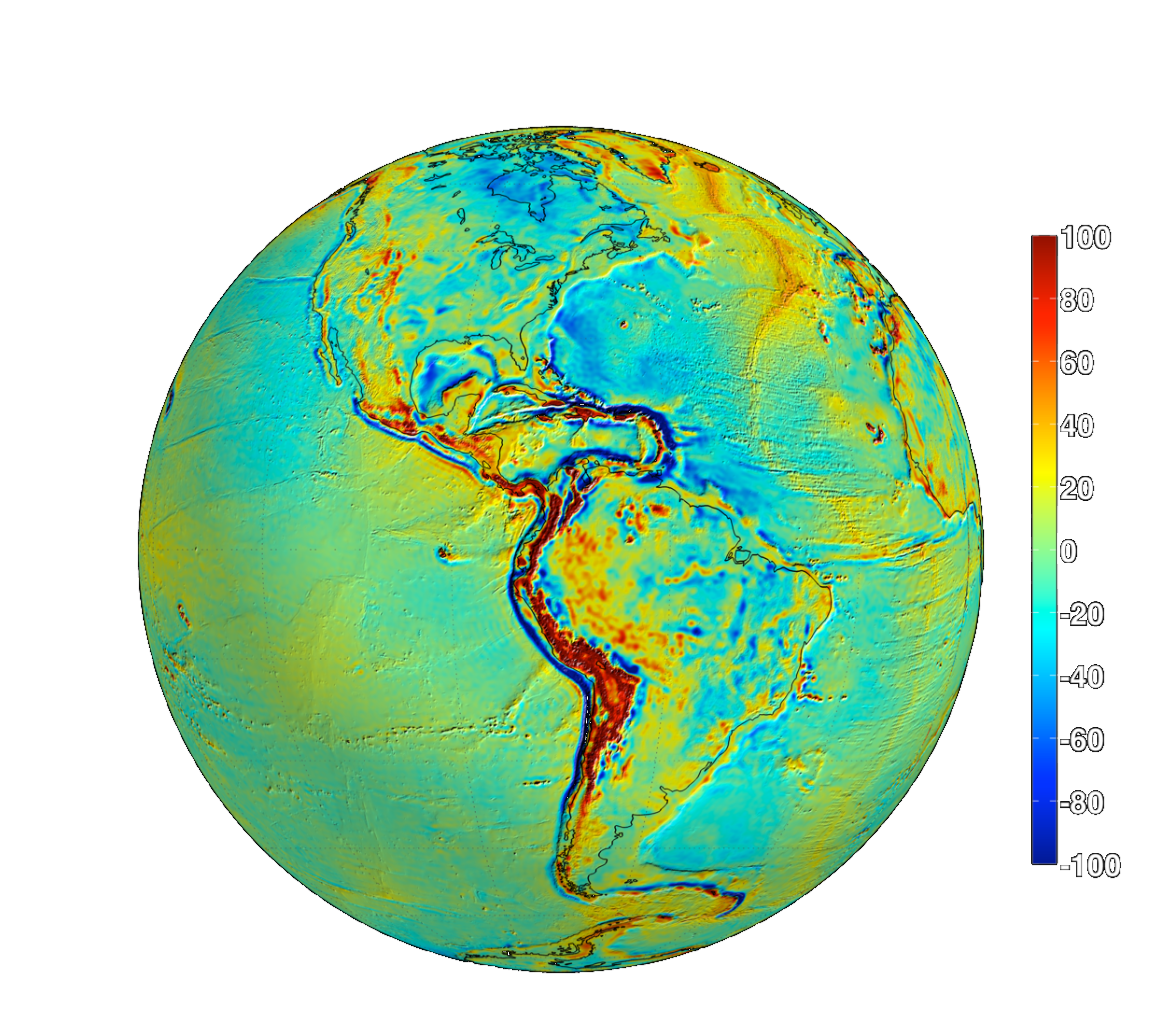
\includegraphics[width=0.99\textwidth]{Figures/Gravity/Exported/Grace_JPLCaltect_FODT10_WithoutPeople.png}
    \end{PointSix}
\end{frame}
    
\begin{frame}
    \begin{PointSix}{Example: Global variability}
    \centering
    \small Your mass is constant but your weight is not.
    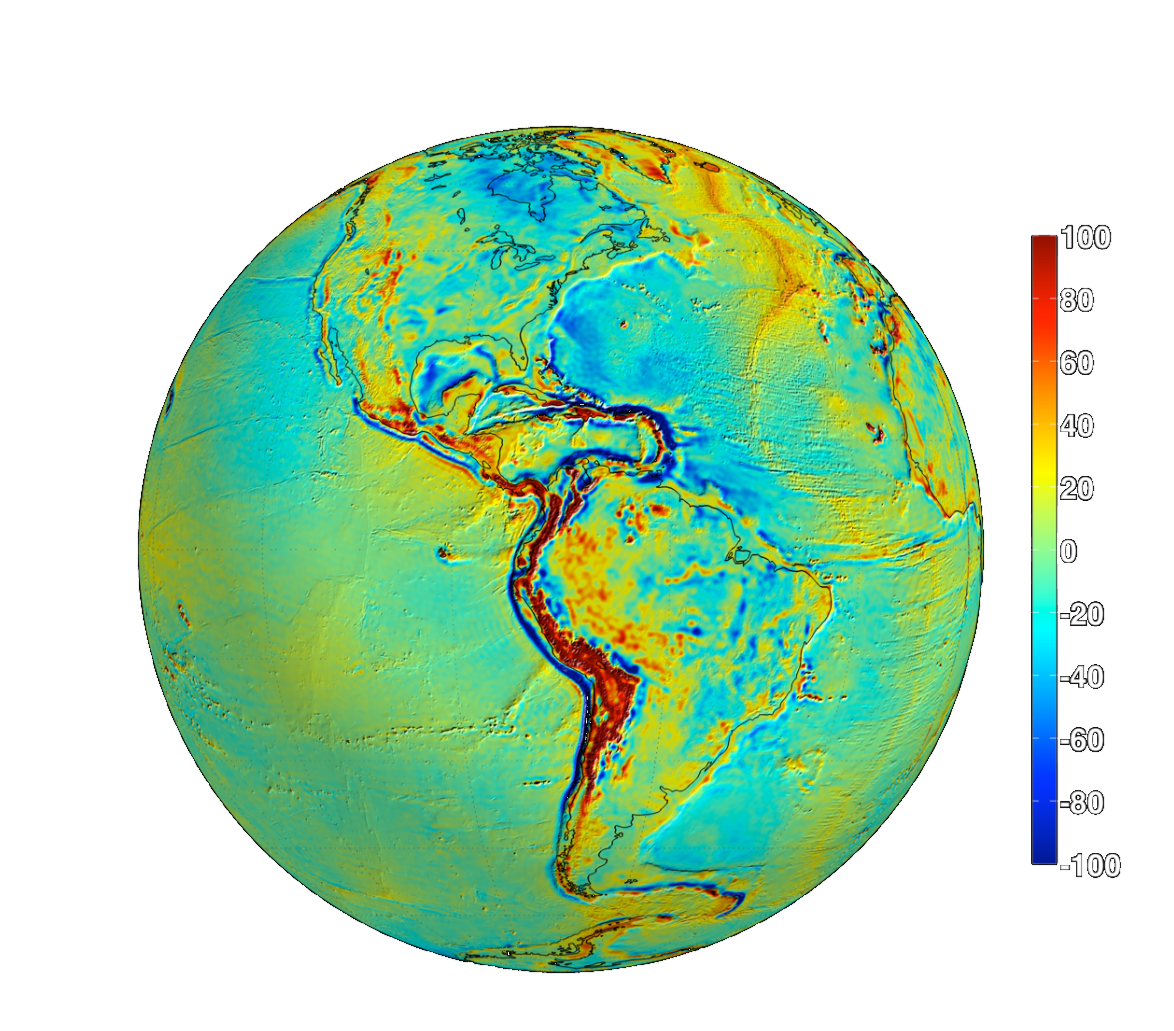
\includegraphics[width=0.99\textwidth]{Figures/Gravity/Exported/Grace_JPLCaltect_FODT10_WithPeople.png}
    \end{PointSix}
\end{frame}
    

\begin{frame}
\begin{ThreeCols}{What is a force?}{
    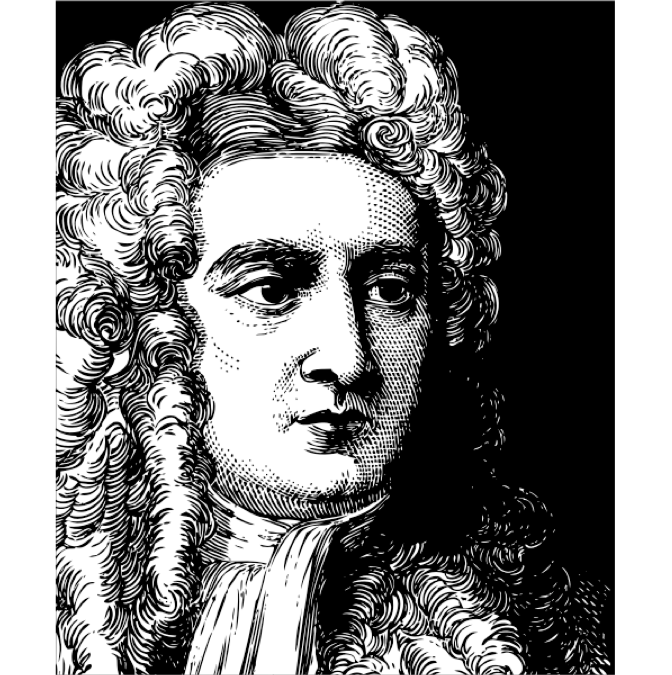
\includegraphics[width=0.8\textwidth]{Figures/Gravity/Exported/Newton_PD_GJohnson.png} \centering \tiny [Newton (1642-1726) / G. Johnson.]}
    \scalebox{1.5}{%
        $
        \vec{F} = m \vec{g}
        $
    }
    \scalebox{0.6}{\parbox{\linewidth}{
        \begin{align*}
        &\vec{F}:\,\text{Force}\,(\text{N};\,\text{kg}\,\text{m}\,\text{s}^{-2})\\
        &\vec{a}:\,\text{Acceleration}\,(\text{m}\,\text{s}^{-2})\\
        &\text{m}:\,\text{Mass (kg)}
        \end{align*}
    }}
\end{ThreeCols}
\end{frame}

\begin{frame}
    \begin{ThreeCols}{The gravitational force}{
        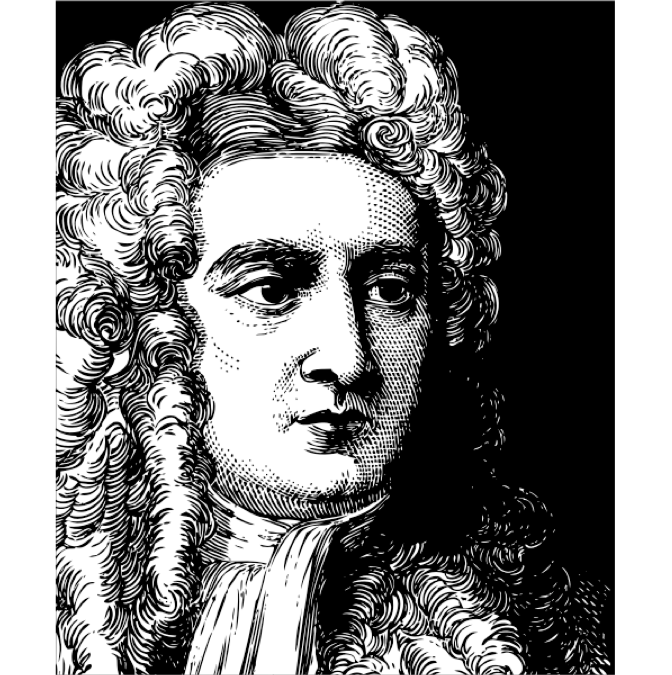
\includegraphics[width=0.8\textwidth]{Figures/Gravity/Exported/Newton_PD_GJohnson.png} \centering \tiny [Newton (1642-1726) / G. Johnson.]}
        \scalebox{1.5}{%
            $
            \vec{F} = G\frac{mM}{r^2}\hat{r}
            $
        }
        \scalebox{0.6}{\parbox{\linewidth}{
            \begin{align*}
            &G=6.674 \cdot 10^{-11}\,\text{(}\,m^3 kg^{-1} s^{-2}\text{)}\\
            &\hat{r}:\,\text{unit vector}\\
            &r:\,\text{distance between point masses}
            \end{align*}
        }}
        \begin{tikzpicture}
            \coordinate (A) at (1,2);
            \coordinate (B) at (2,4);
            
            \draw [fill=white] (A) circle (8pt) node [left,xshift=-0.5cm] {M};
            \draw [fill=white] (B) circle (4pt) node [left,xshift=-0.5cm] {m};
            
               
            \draw[-latex,thick,Karminrot,->] (A) -- (B) node[midway,left,rotate=0] {$r$};
            \draw [-latex,thick, Karminrot] (B) -- (A);
            \end{tikzpicture}
    \end{ThreeCols}
    \end{frame}

    \begin{frame}
        \begin{PointSix}{Example: The gravitational constant}
            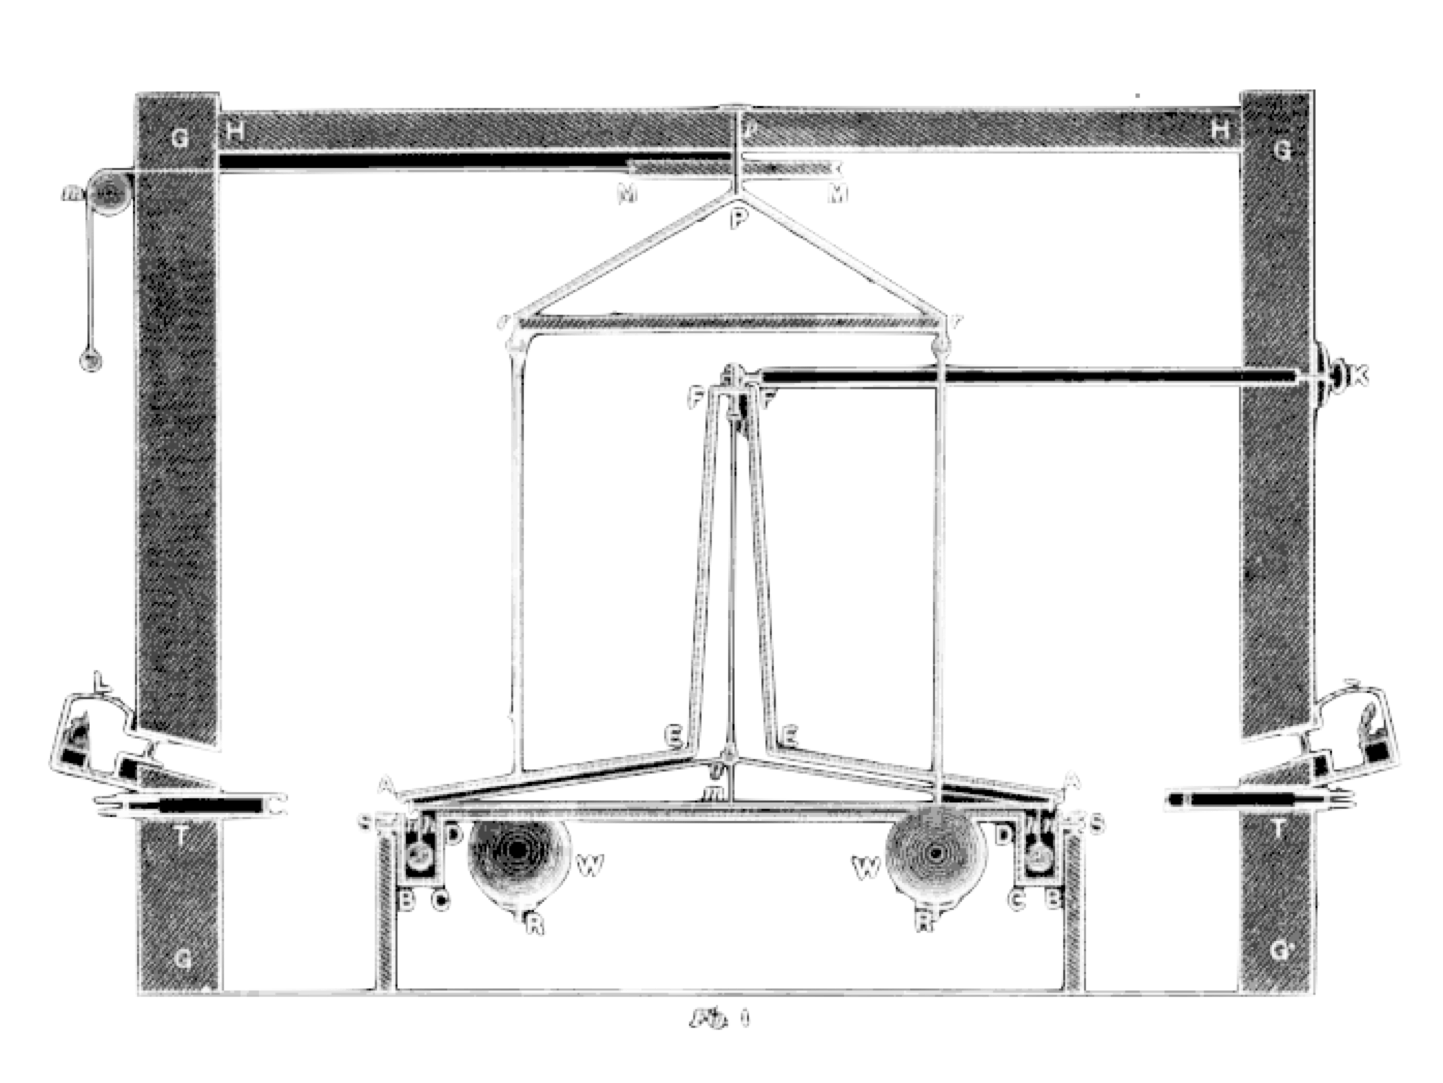
\includegraphics[width=0.99\textwidth]{Figures/Gravity/Exported/Cavendish_PNAS1798.png}
            \centering
            \tiny Cavnedish, PNAS, 1798
        \end{PointSix}
    \end{frame}
    \begin{frame}
        \begin{PointSix}{Example: The gravitational constant}
            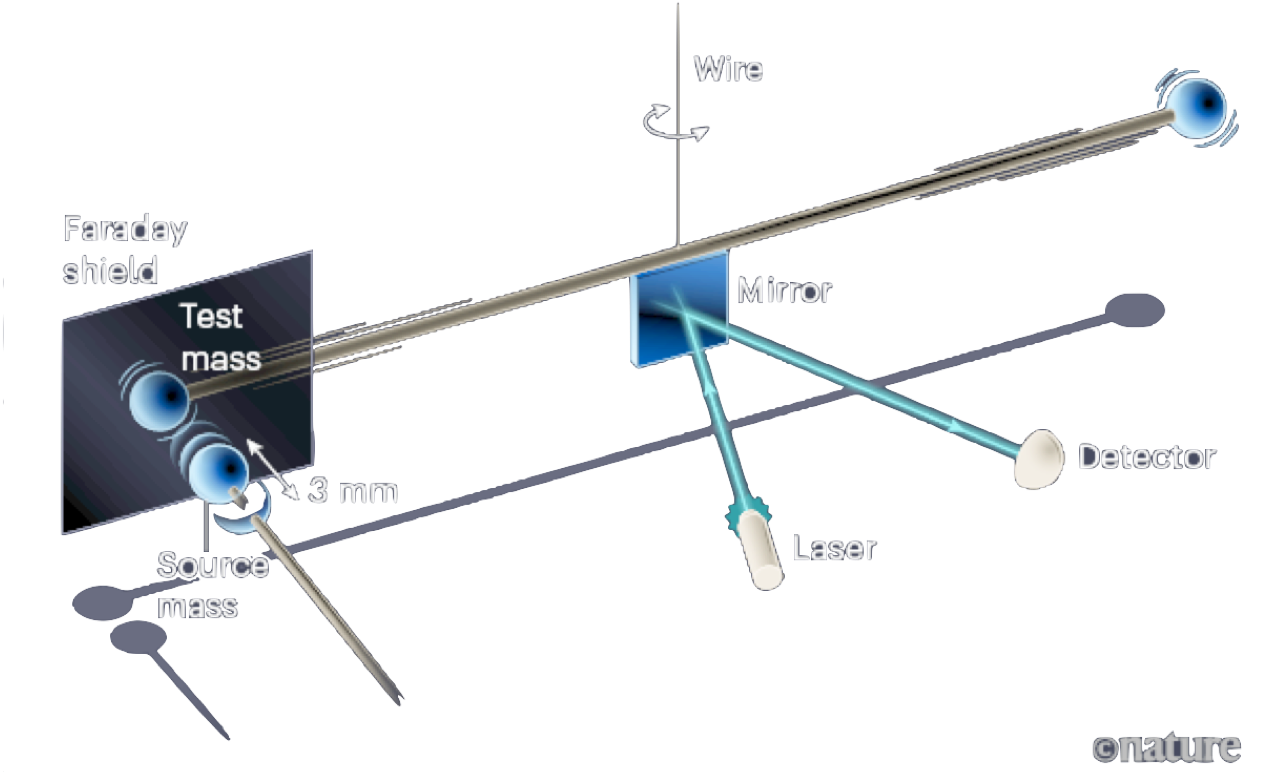
\includegraphics[width=0.99\textwidth]{Figures/Gravity/Exported/MeasuringG_Westphal_Nature2021.png}
            \centering
            \tiny Westphal et al., Nature, 2021
        \end{PointSix}
    \end{frame}   

\begin{frame}
    \frametitle{sadfsd}
    sdf
    % \begin{python}
    %     \begin{figure}
    %     \centering
    %     \begin{python}
    %     #
    %     from pyx import *
        
    %     g = graph.graphxy(width=8)
    %     g.plot(graph.data.function("y(x)=sin(x)/x", min=-15, max=15))
    %     g.writePDFfile("function")
    %     print r'\includegraphics{function}'
    %     \end{python}
    %     \caption{$y(x)=\frac{\sin(x)}{x}$}
    %     \end{figure}
    % \end{python}
    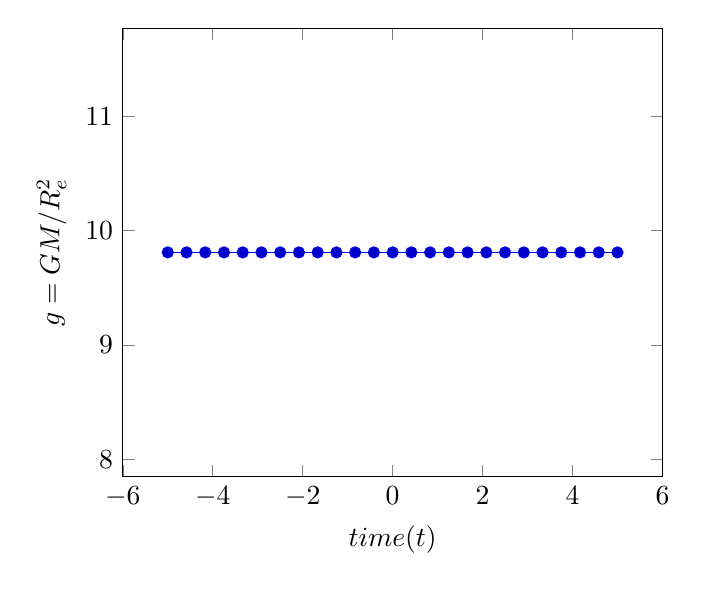
\begin{tikzpicture}
        \begin{axis}[ 
          xlabel=$time (t)$,
          ylabel={$g = G M/R_e^2$}
        ] 
          \addplot {x*0 +9.81}; 
        \end{axis}
      \end{tikzpicture}
\end{frame}

% &\vec{F} = G\frac{mM}{r^2}\hat{r}


% &G=6.674 \cdot 10^{-11}\,\text{(}\,m^3 kg^{-1} s^{-2}\text{)}\\\
% &\hat{r}:\,\text{unit vector pointing into the direction of force}\\
% &r:\,\text{distance between mass } M \text{and mass } m



  \end{document}​